\documentclass[12pt, letter, oneside]{book}
\usepackage{fancyhdr, ifpdf}
\usepackage{float}
\usepackage{setspace}
\usepackage{color}
\usepackage{xcolor}
\usepackage{listings}
\usepackage{caption}
\usepackage[ampersand]{easylist}
\usepackage{amssymb}
\usepackage{pdflscape}
\usepackage{verbatim}
\usepackage{longtable}
\usepackage[margin=1cm]{caption}
\usepackage[top=1in, bottom=.75in, left=.7in, right=1in]{geometry}
\ListProperties(Hide=100, Hang=true, Progressive=3ex,Style*=$\bullet$ , Style2*=-- )

\definecolor{mygray}{rgb}{0.9,0.9,0.9}
\lstdefinestyle{customc}{
  backgroundcolor=\color{mygray},
  captionpos=b, 
  belowcaptionskip=1\baselineskip,
  breaklines=true,
  numbers=left,
  numberstyle=\footnotesize,
  %frame=L,
  xleftmargin=\parindent,
  language=C++,
  showstringspaces=false,
  basicstyle=\footnotesize\ttfamily,
  keywordstyle=\bfseries\color{green!40!black},
  commentstyle=\itshape\color{purple!40!black},
  identifierstyle=\color{black},
  stringstyle=\color{cyan}  
}

\lstset{escapechar=@,style=customc,tabsize=4}

%% some redefination of the headers and footers
\renewcommand{\chaptermark}[1]%
                 {\markboth{#1}{}}
\renewcommand{\sectionmark}[1]%
                 {\markright{\thesection\ #1}}
\lhead[\fancyplain{}{\thepage}]%
      {\fancyplain{}{\rightmark}}
\rhead[\fancyplain{}{\leftmark}]%
      {\fancyplain{}{\thepage}}
\cfoot{}
\sloppy

\ifpdf
   \usepackage[pdftex]{graphicx}
   \usepackage{rotating}
\else
   \usepackage{graphicx}
	\usepackage{rotating}   
\fi

\graphicspath{{./Figures/}}
\doublespacing

\begin{document}
\doublespace

\clearpage
\pagenumbering{arabic}

\setcounter{chapter}{0}

\chapter*{Parameter Minimization using the Nelder-Mead algorithm}
\setcounter{chapter}{1}
\emph{Do some fitting}
\section{Introduction}
The Nelder-Mead plugin is used to fit a SBML models parameters to experimental data. 

The plugin has numerous properties to allow the user full control over the internal fitting engine, as well as 
access to generated fitted data after a minimization session. In addition, various statistical properties, such as standardized residuals, Q-Q data, ChiSquare and reduced ChiSquare are made accessible to the user. The resulting parameter values do also come with estimated confidence limits.

The current implementation is based on the Nelder-Mead C implementation by Michael F. Hutt\footnote{ 

 An implementation of the Nelder-Mead simplex method. 
 Copyright (c) 1997-2011 Michael F. Hutt
}.


Plugin properties are documented in the next section.

\begin{landscape}
\section{Plugin Properties}
Available properties in the Nelder-Mead plugin are listed in the table below.

%\begin{table}[ht]
\centering % used for centering table
\begin{longtable}{p{4cm} l p{3cm}  p{10cm}} % centered columns 

Property Name & Data Type & Default Value  & Description \\ [0.5ex] % inserts table 
%heading
\hline % inserts single horizontal line
SBML                            &   string              & N/A    &   SBML document as a string. Model to be used in the fitting. \\
ExperimentalData   				&	telluriumData 		& N/A    &   Input data.  \\
FittedData      				& 	telluriumData    	& N/A    &   Output data. \\
InputParameterList 				&	listOfProperties    & N/A    &   Parameters to fit. \\
OutputParameterList 			&   listOfProperties 	& N/A    &   List of fitted parameters. \\
Experimental\-DataSelectionList & 	stringList			& N/A    &   Species selection list for experimental data. \\
FittedDataSelectionList     	& 	stringList			& N/A    &   Selection list for model data. \\
Norm							&	double				& N/A    &   Norm of fitting. An estimate of goodness of fit. \\
Norms							&	telluriumData		& N/A    &   The norm is calculated throughout a fitting session. Each Norm value is stored in the 	\verb|Norms| (read-only) property. \\

ConfidenceLimits				&	listOfProperties	& N/A    &   Confidence limits for each fitted parameter. The confidence limits are calculated at a 95\% confidence level. \\

Hessian							&	matrix				& N/A    &   Hessian matrix. The Hessian is calculated using approximation at a found parameter minimum. \\
CovarianceMatrix				&	matrix				& N/A    &   Covariance matrix. Calculated as the inverse of the Hessian.\\
Residuals     					& 	telluriumData    	& N/A    &   Residuals data.  \\
StandardizedResiduals			&	telluriumData		& N/A    &   Standardized Residuals.\\
NormalProb\-abilityOfResiduals	&	telluriumData		& N/A    &   Normal Probability of Residuals.\\
ChiSquare						&	double				& N/A    &   The ChiSquare at the minimum.\\
ReducedChiSquare				&	double				& N/A    &   The Reduced ChiSquare at the minimum.\\
StatusMessage					&	string				& N/A    &   Message from the internal fitting engine, communicating the status of the obtained fit (Currently not used).\\
NrOfIter                        &   int                 & N/A    &   Number of (internal outer loop) iterations. \\
NrOfFuncIter                    &   int                 & N/A    &   Number of objective function iterations. \\
\\[2pt]                                                               
\multicolumn{4}{p{19cm}}{The following properties are used internally by the fitting engine. They are preset with default values. Depending on the minimization problem at hand, they may need to be tweaked. } \\[12pt]
\hline %inserts single line                                           
\\[2pt]                                                               
Epsilon                         &   double              & 1.e-6          		&   Convergence tolerance. \\
Scale                           &   double              & 1			            &   Scaling of vertices. \\
MaxNrOfIterations               &   int		            & 1000          		&   Maximum number of iterations. \\
Alpha                         	&   double              & 1.          			&   Reflection coefficient. \\
Beta                       		&   double              & 0.5                 	&   Contraction coefficient. \\
Gamma                        	&   double              & 1                   	&   Expansion coefficient. \\
                                                        
\hline %inserts single line                             
\caption{Plugin Properties} 
\label{table:nmPluginProperties} 
\end{longtable}
%\end{table}

\end{landscape}

\section{Plugin Events}
The Nelder-Mead plugin are using all of a plugins available plugin events, i.e. the \emph{PluginStarted}, \emph{PluginProgress} and the \emph{PluginFinished} events.

The available data variables for each event are internally treated as \emph{pass trough} variables, so any data, for any of the events, assigned prior to 
the plugins execute function (in the assingOn.. family of functions), can be retrieved unmodified in the corresponding event function.

\begin{table}[ht]
\centering % used for centering table
\begin{tabular}{l l p{9cm}} 

Event & Arguments & Purpose and argument types \\ [0.5ex] % inserts table 
%heading
\hline % inserts single horizontal line
PluginStarted  	& 	void*, void*  & Signal to application that the plugin has started. Both parameters are \emph{pass trough} parameters and are unused internally by the plugin.\\[0.5ex]
PluginProgress	& 	void*, void*  & Communicating progress of fitting. Both parameters are \emph{pass trough} parameters and are unused internally by the plugin. \\[0.5ex]
PluginFinished	& 	void*, void*  & Signals to application that execution of the plugin has finished. Both parameters are \emph{pass trough} parameters and are unused internally by the plugin.\\

\hline %inserts single line
\end{tabular}
\caption{Plugin Events} 
\label{table:nmPluginEvents} 
\end{table}

\section{Python example}
The following Python script illustrate how the plugin can be used. 

\begin{singlespace}
\lstinputlisting[label=NelderMeadExample,caption={Minimization example.},language=Python]{Examples/telNelderMead.py}
\end{singlespace}

\begin{sidewaysfigure}
\centering
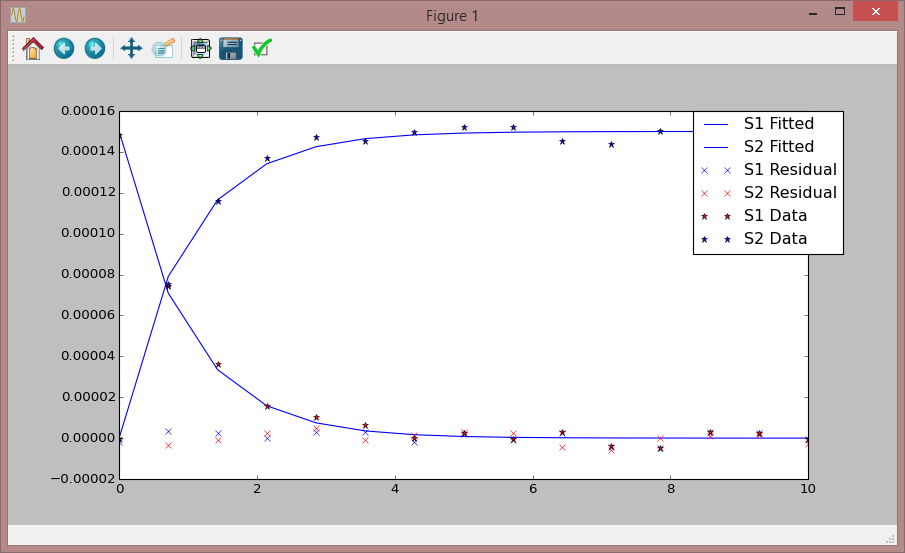
\includegraphics[width=220mm]{NelderMeadOutput.png}
\caption{Typical output for the example script above.}
\label{fig:nmFig}
\end{sidewaysfigure}








\end{document}






